% Created 2017-01-10 Tue 23:08
\documentclass[10pt]{article}
\usepackage[utf8]{inputenc}
\usepackage[T1]{fontenc}
\usepackage{fixltx2e}
\usepackage{graphicx}
\usepackage{longtable}
\usepackage{float}
\usepackage{wrapfig}
\usepackage{rotating}
\usepackage[normalem]{ulem}
\usepackage{amsmath}
\usepackage{textcomp}
\usepackage{marvosym}
\usepackage{wasysym}
\usepackage{amssymb}
\usepackage{hyperref}
\tolerance=1000
\usepackage{minted}
\author{Karolina Ziomek, Rasmus Holm}
\date{\today}
\title{Big Data Analytics \\ 732A54 \\ Lab 5}
\hypersetup{
  pdfkeywords={},
  pdfsubject={},
  pdfcreator={Emacs 25.1.1 (Org mode 8.2.10)}}
\begin{document}

\maketitle
\newpage

\section*{Temperature Kernel}
\label{sec-1}
In this lab we were supposed to implement a kernel to predict temperatures. 
The kernel is a linear combination of three Gaussian kernels, one taking the date into consideration,
one using the time of day, and the last uses the geographical distance.

The estimated temperatures below were predicted in Linköping 2013-06-24. We can see the shape is reasonable,
lower temperatures in the morning and evening with a peak in the afternoon. However, the values of the temperatures
are not particular realistic, even for Sweden, in the middle of the summer. This indicates that the kernel does
not consider seasonal trends and it turns out that changing the date does not change the estimated values very much.

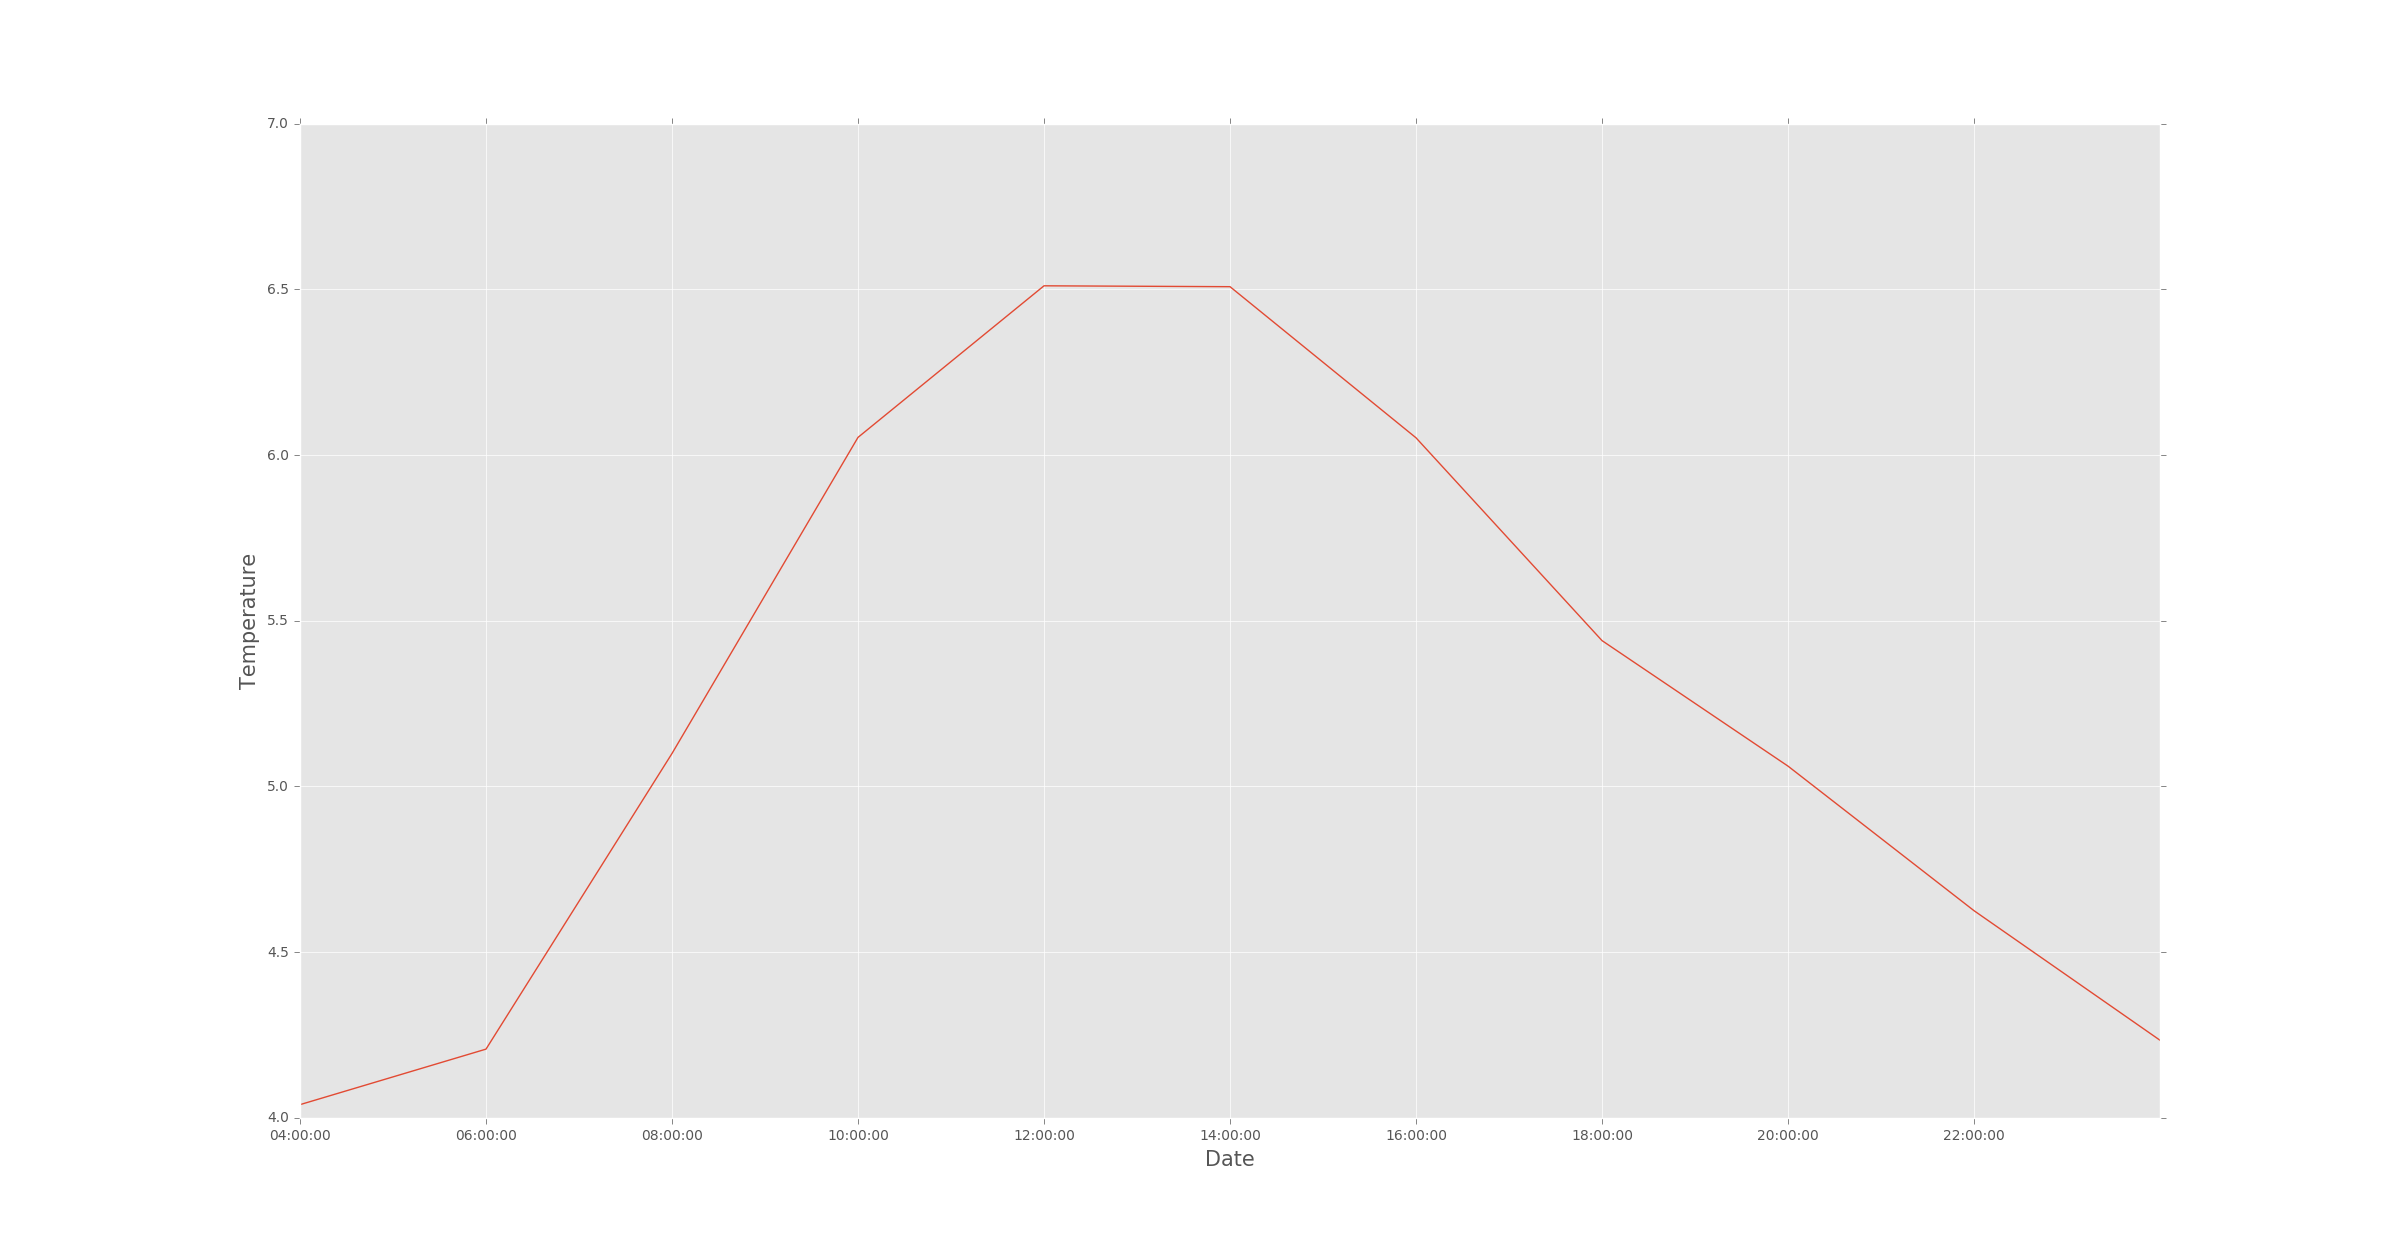
\includegraphics[width=\textwidth]{./images/estimated_temps.png}

We can gain some insight to what is wrong with our kernel from the plots below that show the distances and the kernel weights.

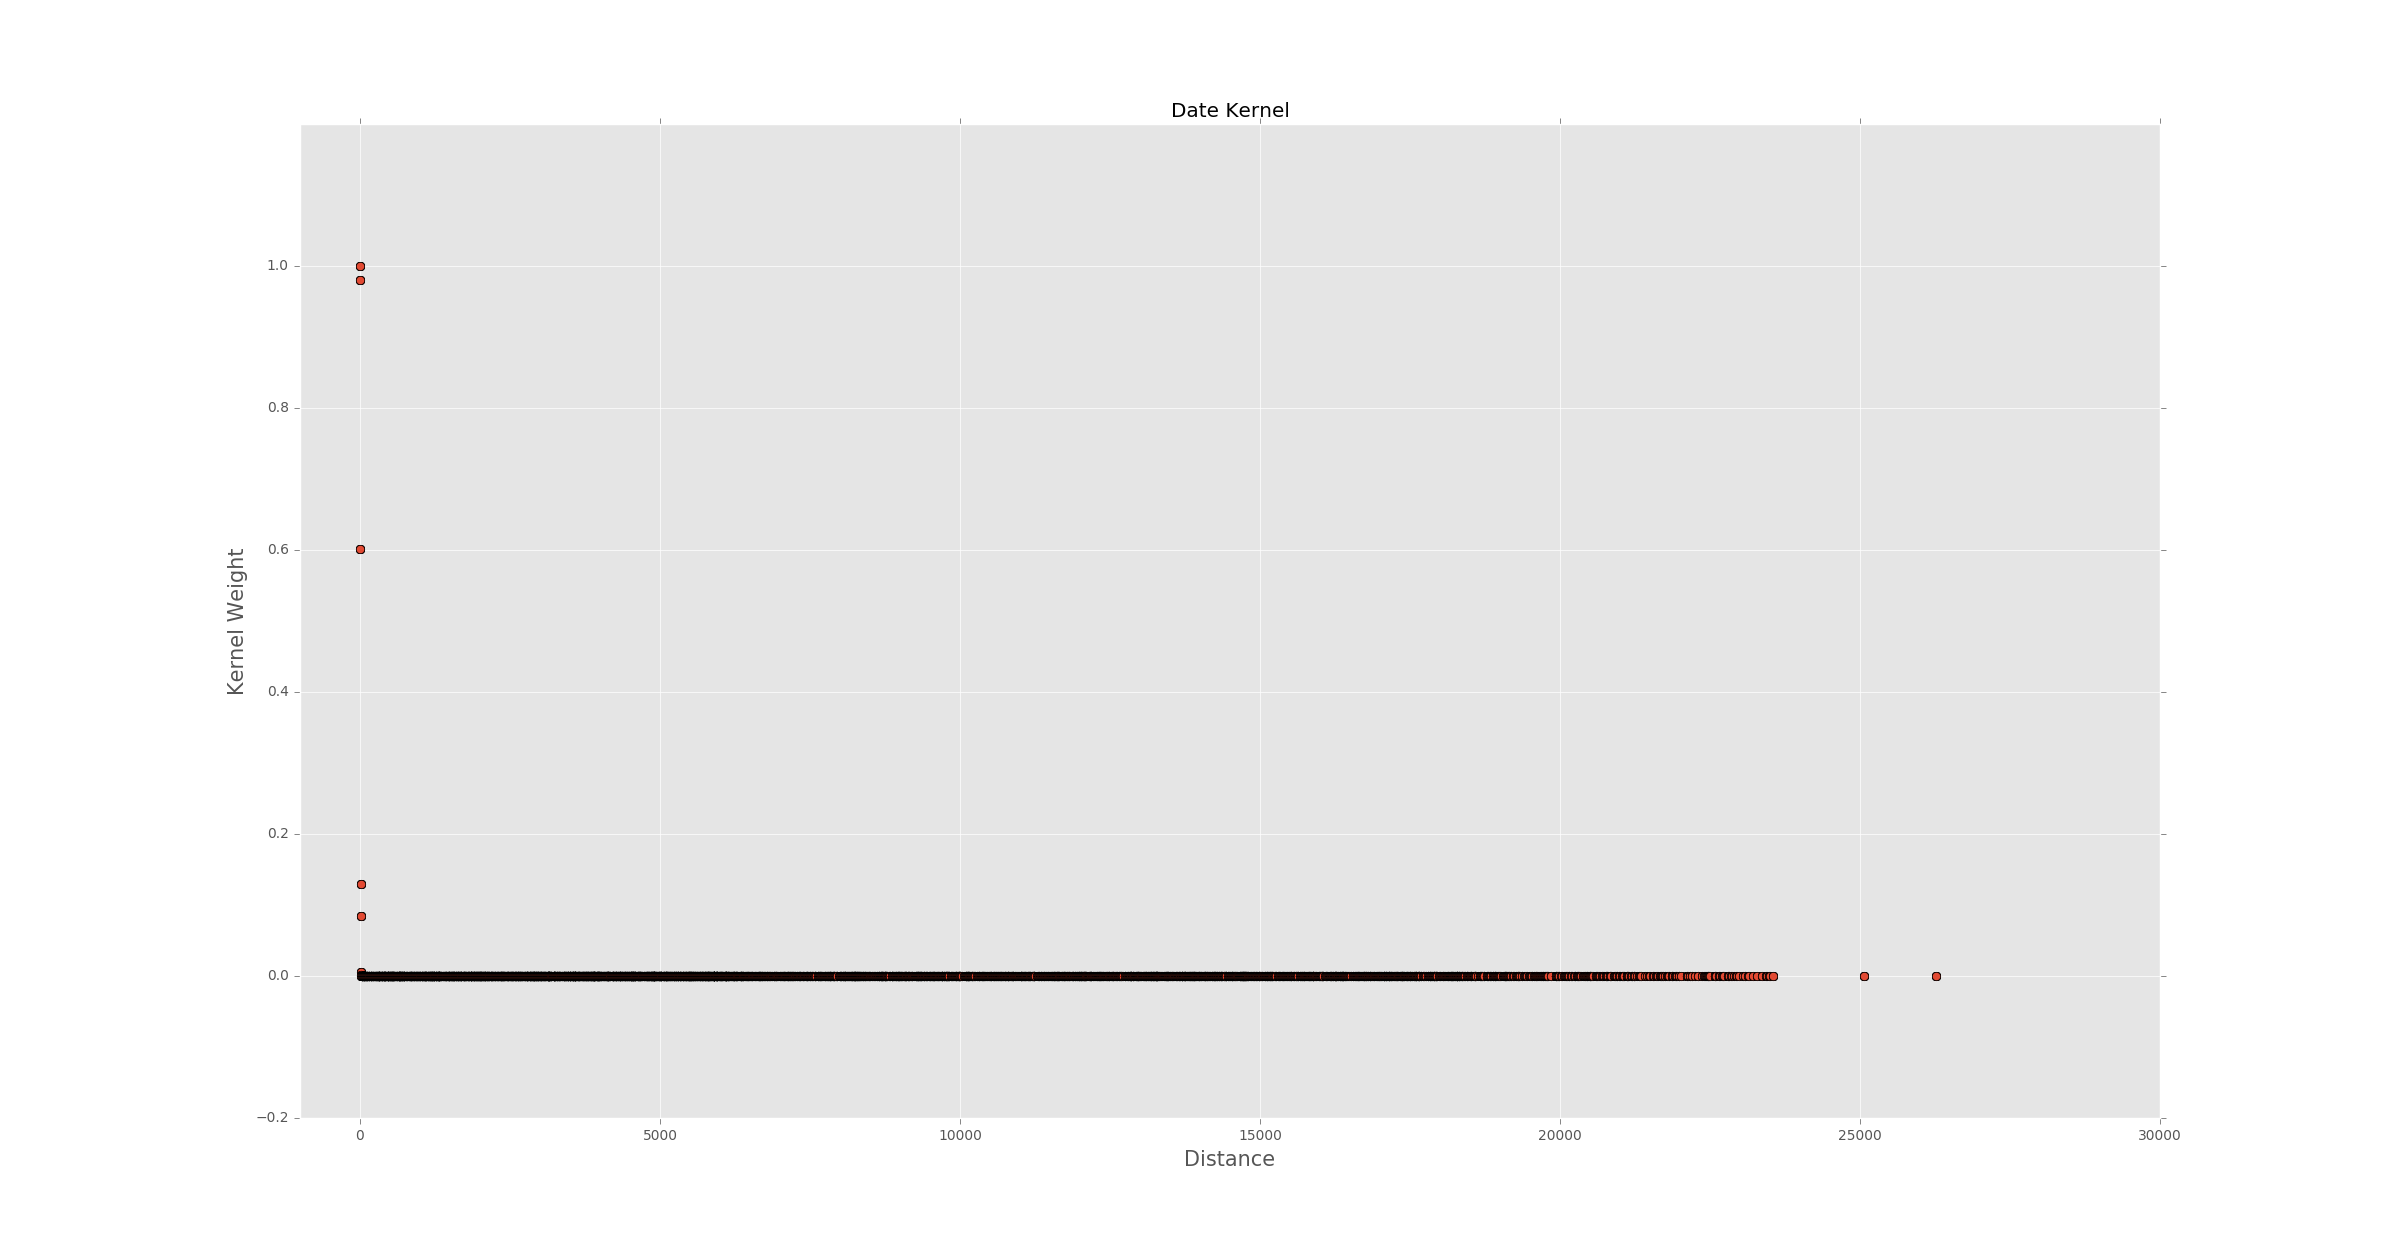
\includegraphics[width=\textwidth]{./images/date_kernel.png}

From the date kernel above we can see that only a few observations have a weight above 0 and that is what we wanted
by picking the width of 7. It is reasonable to assume that the temperature of a particular day 
is similar to what it has been the 7 previous days. However, since we added the kernels together they are independent
of each other and since the date kernel only has a few number of contributing observations it will not be particular influential in the
prediction.

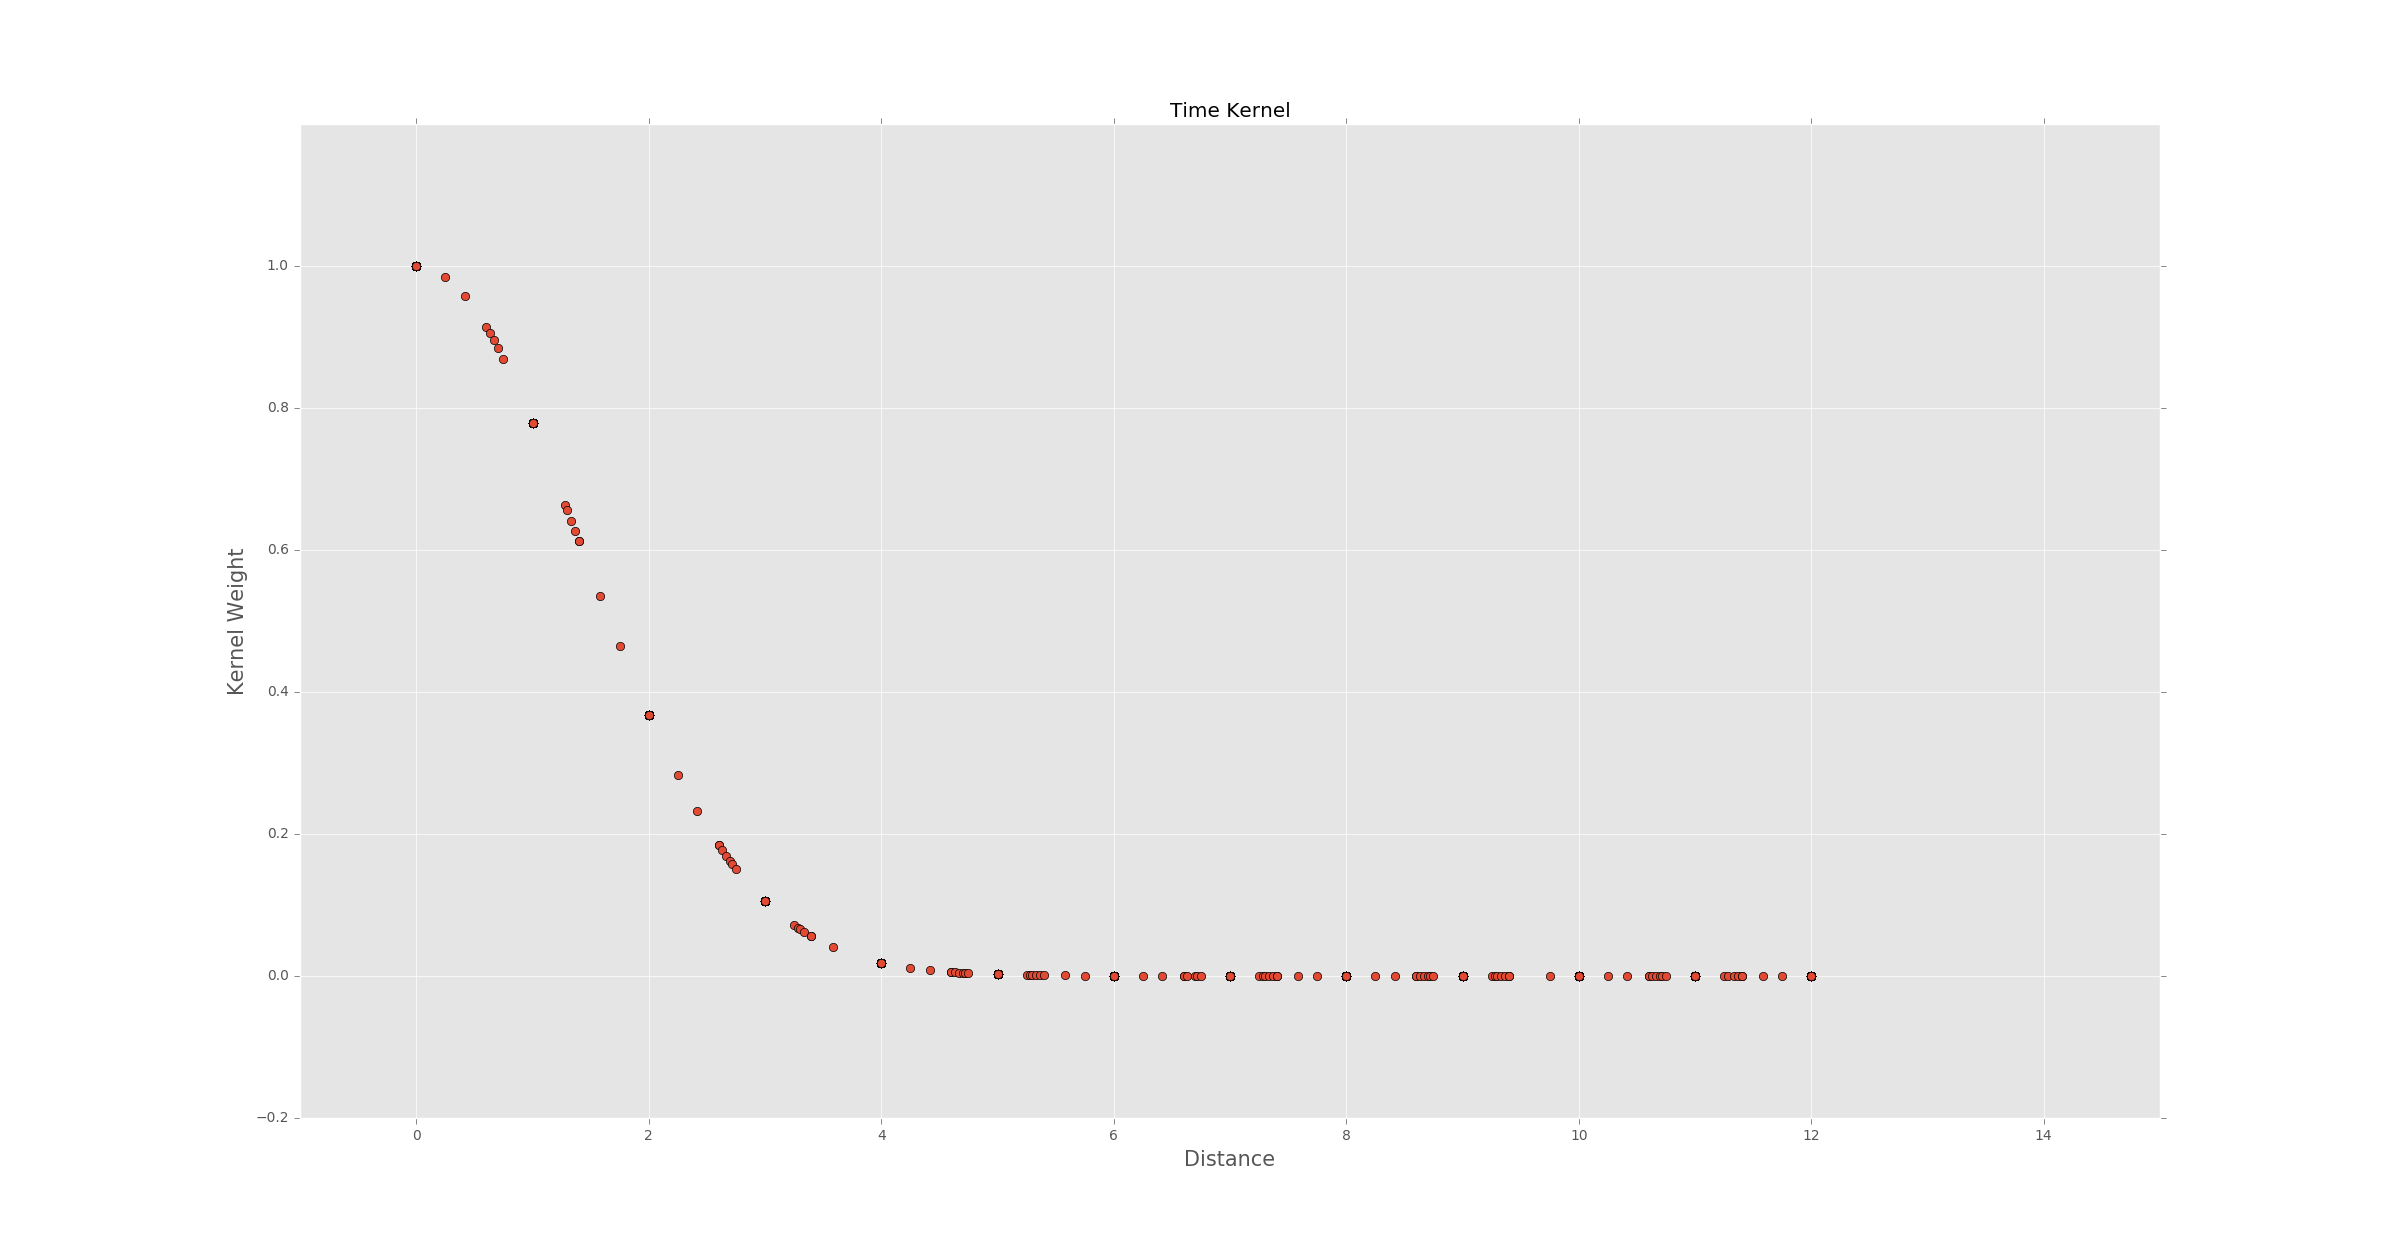
\includegraphics[width=\textwidth]{./images/time_kernel.png}

We picked the width of the time kernel to be 2 since the last few hours should have a similar temperatures as the current time.
We can observe that only observations within about 4 hours time have weights above 0 which we think is reasonable.

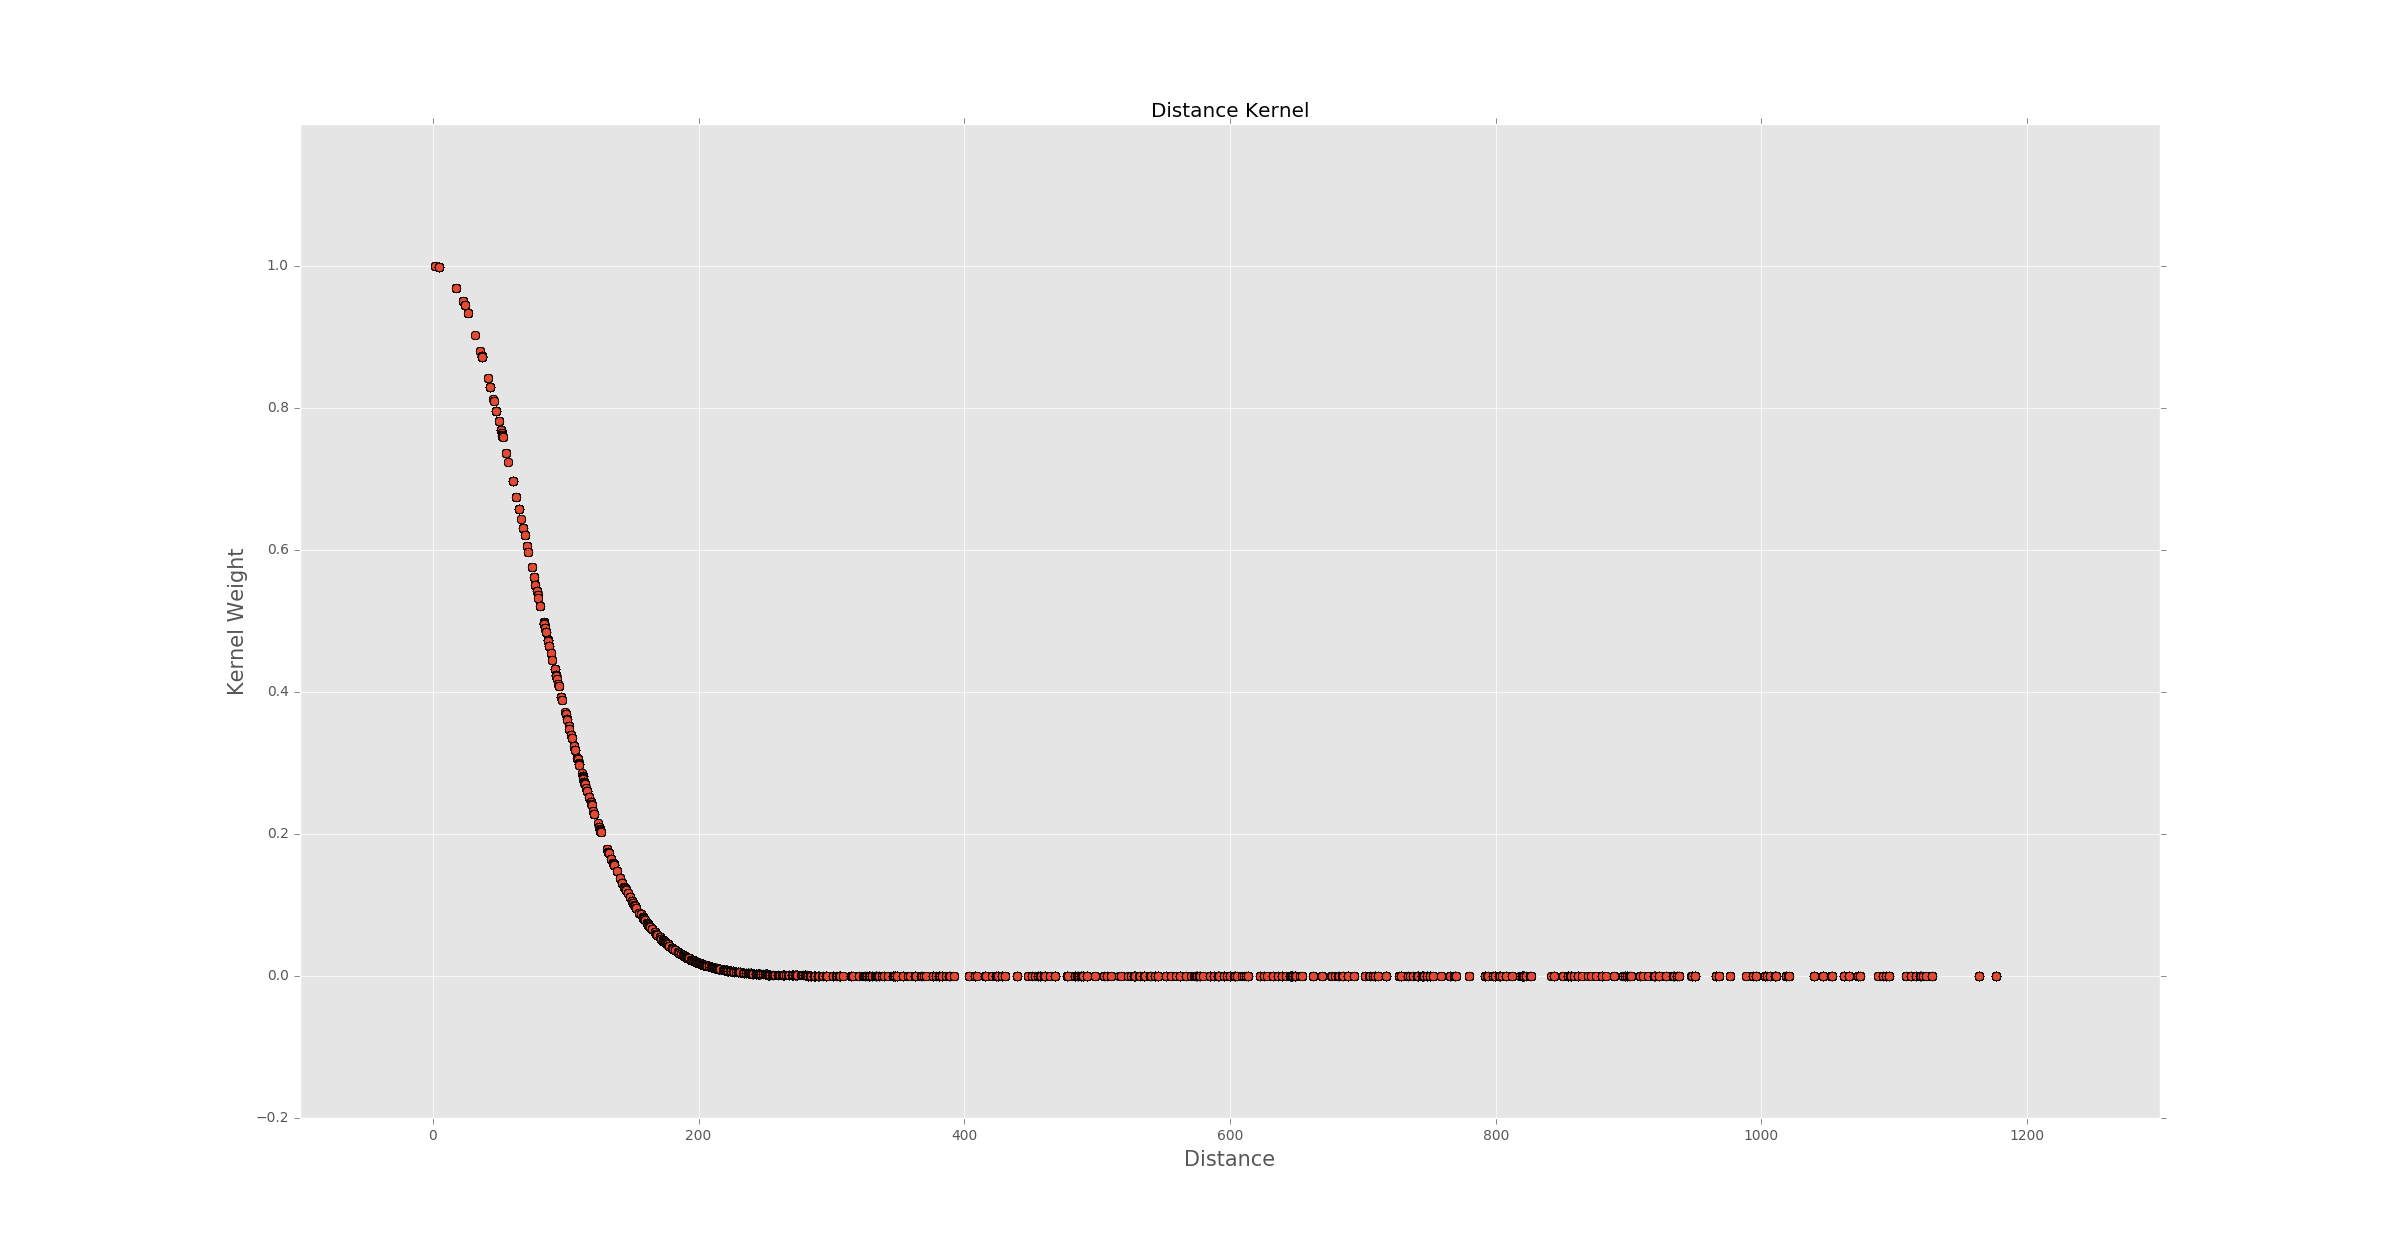
\includegraphics[width=\textwidth]{./images/distance_kernel.png}

For the distance kernel we picked a width of 100 to transform the kilometers to 10 Swedish miles which we thought was a
good measure based on the size of Sweden. Location affects the temperature quite much, the further to the north the colder
it usually gets. We can see that weights above 0 are restricted to observations within a circle with a radius of roughly 200 kilometers. 

We have stated it before, the main problem with the kernel is that the different kernels are independent of each other.
The date kernel is the only kernel that can detect seasonal trends but given the independence it cannot contribute much
to the prediction. Had the kernels been multiplied together the predictions would probably have had been much better
since the date kernel would 0 out the other kernels where its weight is 0. This would give only the few last days
predictive power. As of now the kernel basically averages all the temperatures at a specific time over all the years
in a radius of 200 kilometers as its prediction.

To create a better kernel the simplest solution would be to multiply them together but it would probably not be a particular
good estimator. Another suggestion would be to create a multivariate Gaussian kernel which of course would be a harder
problem to solve but the covariance matrix could possibly represent more accurate correlations.

\section*{Code}
\label{sec-2}
\begin{minted}[]{python}
from __future__ import division
from math import radians, cos, sin, asin, sqrt, exp
from datetime import datetime
from pyspark import SparkContext

if not "sc" in locals() or not "sc" in globals():
    sc = SparkContext()

def haversine(lon1, lat1, lon2, lat2):
    """
    Calculate the great circle distance between two points
    on the earth (specified in decimal degrees)
    """
    # convert decimal degrees to radians
    lon1, lat1, lon2, lat2 = map(radians, [lon1, lat1, lon2, lat2])
    # haversine formula
    dlon = lon2 - lon1
    dlat = lat2 - lat1
    a = sin(dlat/2)**2 + cos(lat1) * cos(lat2) * sin(dlon/2)**2
    c = 2 * asin(sqrt(a))
    km = 6367 * c
    return km

def kernel_model():
    h_distance = 100
    h_date = 7
    h_time = 2

    pred_latitude = 58.409158
    pred_longitude = 15.607452

    pred_date = datetime.strptime("2013-06-24", "%Y-%m-%d")
    pred_times = [datetime.strptime(time, "%H:%M:%S")
                  for time in ["04:00:00", "06:00:00", "08:00:00", "10:00:00",
                               "12:00:00", "14:00:00", "16:00:00", "18:00:00",
                               "20:00:00", "22:00:00", "00:00:00"]]

    stations = sc.textFile("/user/x_rahol/data/stations.csv")
    temps = sc.textFile("/user/x_rahol/data/temperature-readings.csv")

    # (station, (latitude, longitude))
    stations = stations.map(lambda line: line.split( ",")) \
                       .map(lambda obs: (int(obs[0]),
                                         (float(obs[3]),
                                          float(obs[4]))))

    # (station, (date, time, temperature))
    temps = temps.filter(lambda line: len(line) > 0) \
                 .map(lambda line: line.split(";")) \
                 .map(lambda obs: (int(obs[0]),
                                   (datetime.strptime(obs[1], "%Y-%m-%d"),
                                    datetime.strptime(obs[2], "%H:%M:%S"),
                                    float(obs[3]))))

    station_positions = stations.collectAsMap()
    station_positions = sc.broadcast(station_positions).value

    # (station, (longitude, latitude, date, time, temperature))
    combined_data = temps.map(lambda (station, (date, time, temp)):
                              (station, (station_positions[station][1],
                                         station_positions[station][0],
                                         date, time, temp)))
    combined_data.cache()

    result = [combined_data.filter(lambda x:
                                   filter_date(x=x,
                                               date=pred_date,
                                               time=pred_time)) \
              .map(lambda x: (temperature_kernel(x, pred_longitude,
                                                 pred_latitude, h_distance,
                                                 pred_date, h_date,
                                                 pred_time, h_time),
                              get_temp(x))) \
              .map(lambda (kernel, temp):
                   (None, (kernel * temp, kernel))) \
              .reduceByKey(lambda (estimate1, kernel1), (estimate2, kernel2):
                           (estimate1 + estimate2, kernel1 + kernel2)) \
              .map(lambda (key, (estimate, kernel)): (key, estimate / kernel)) \
              .collect()[0][1]
              for pred_time in pred_times]

   sc.parallelize(result) \
     .repartition(1) \
     .saveAsTextFile("/user/x_rahol/result/kernel_result/temps")


def filter_date(x, date, time):
    merged_pred = datetime.combine(datetime.date(date),
                                   datetime.time(time))
    merged_true = datetime.combine(datetime.date(get_date(x)),
                                   datetime.time(get_time(x)))
    return merged_true <= merged_pred

def gaussian_kernel(u):
    return exp(-u**2)

def date_kernel(x, date, h):
    distance = date_distance(x, date)
    return gaussian_kernel(distance / h)

def date_distance(x, date):
    distance = (date - get_date(x)).days
    return distance

def time_kernel(x, time, h):
    distance = time_distance(x, time)
    return gaussian_kernel(distance / h)

def time_distance(x, time):
    seconds_per_hour = 3600
    distance = (get_time(x) - time).seconds / seconds_per_hour

    if distance > 12:
        distance = 24 - distance

    return distance

def distance_kernel(x, longitude, latitude, h):
    distance = distance_distance(x, longitude, latitude)
    return gaussian_kernel(distance / h)

def distance_distance(x, longitude, latitude):
    distance = haversine(get_longitude(x), get_latitude(x),
                         longitude, latitude)
    return distance

def temperature_kernel(x, longitude, latitude, h_dist, date, h_date, time, h_time):
    kernel = (distance_kernel(x, longitude, latitude, h_dist) +
              date_kernel(x, date, h_date) + time_kernel(x, time, h_time))
    return kernel

def get_longitude(x):
    return x[1][0]

def get_latitude(x):
    return x[1][1]

def get_date(x):
    return x[1][2]

def get_time(x):
    return x[1][3]

def get_temp(x):
    return x[1][4]

def main():
    kernel_model()
\end{minted}
% Emacs 25.1.1 (Org mode 8.2.10)
\end{document}
